\section{Durchführung}
\label{sec:Durchführung}

\subsection{Vorbereitende Maßnahmen}
Alle Versuche werden mit Schaltkasten 1 durchgeführt.
Bevor der Versuch durchgeführt werden kann, müssen zunächst die Resonanzfrequenzen der Maschen, beziehungsweise der beiden Schwingkreise,
herausgefunden werden.
Bei der linken Maschen wird die Resonanzfrequenz mit fester Kapazität und variabler Spannungsfrequenz %umbedingt besseren Ausdruck finden
gemessen. Die Resonanzfrequenz der rechten Masche wird mit einer festen Spannungsfrequenz und variabler Kapazität  gemessen.
Die Schaltung wird gemäß \autoref{fig:schaltung0} aufgebaut.
\begin{figure}[H]
    \centering
    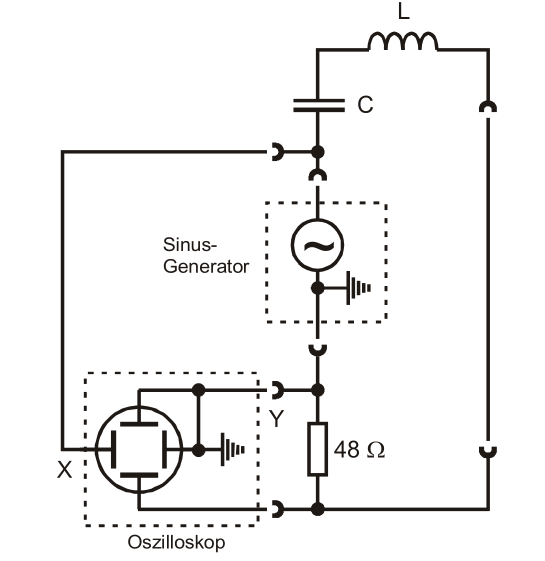
\includegraphics[width=0.75\textwidth]{plots/Schaltung0.png}
    \caption{Schaltung zur Einstellung der Resonanzfrequenz \cite{Versuchsanleitung}}
    \label{fig:schaltung0}
\end{figure}

\noindent Mithilfe eines Generators wird eine Sinusspannung angelegt, die  für die Kreisfrequenz $\omega$ im linken Schwingkreis sorgt. 
Über Lissajous-Figuren, die man über den XY-Betrieb am Oszilloskop erstellt, kann die Phasenverschiebung von dem Generator und 
dem Schwingkreis auf null gesetzt werden. Ist die Lissajous-Figur eine Gerade, dann sind die beiden eingehenden Signale, hier der
Generator und der Schwingkreis, in Phase. Ein Beispiel dafür ist die \autoref{fig:Lissajous}.
\begin{figure}[H]
    \centering
    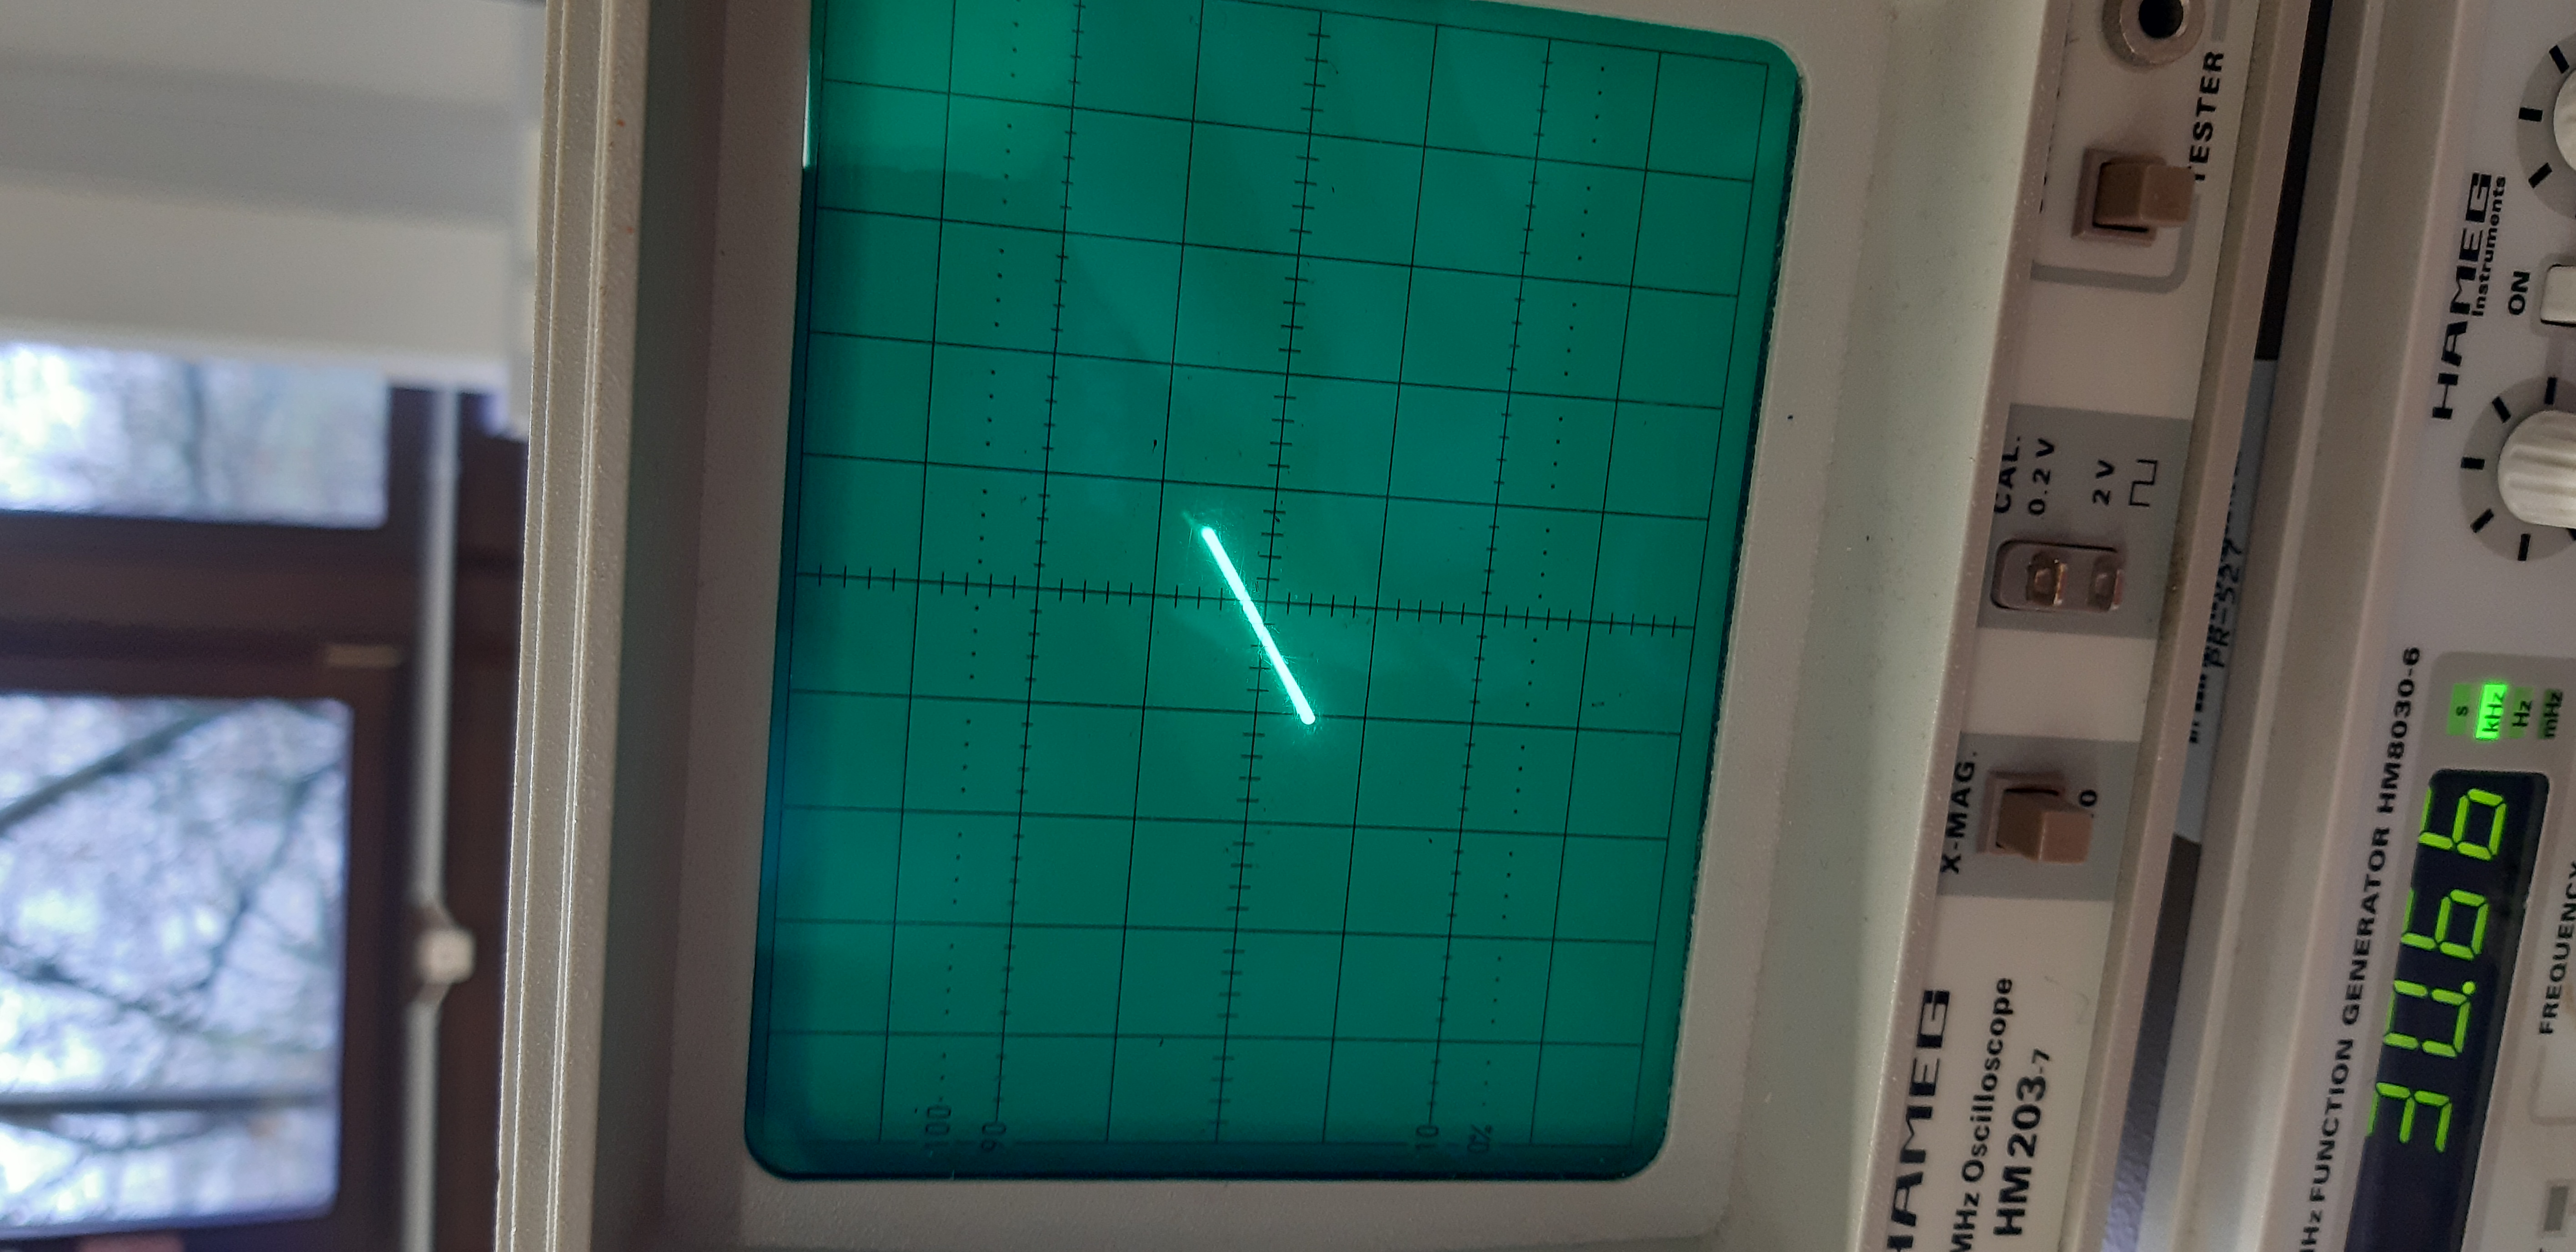
\includegraphics[width=0.75\textwidth, angle=-90]{plots/Lissajour-Gerade.jpeg}
    \caption{Lissajous-Figur der Justierung.}
    \label{fig:Lissajous}
\end{figure}

\noindent Es wird die Resonanzfrequenz der linken Masche festgehalten und auch für die rechte Masche eingestellt, indem die variable Kapazität
des rechten Schwingkreises verstellt wird. Dabei wird die verstellbare Kapazität an dem Schaltkasten so eingestellt, dass die Lissajous-Figur Phasengleichheit 
angibt.

\subsection{Austausch der Schwingungsenergie}
\begin{figure}[H]
    \centering
    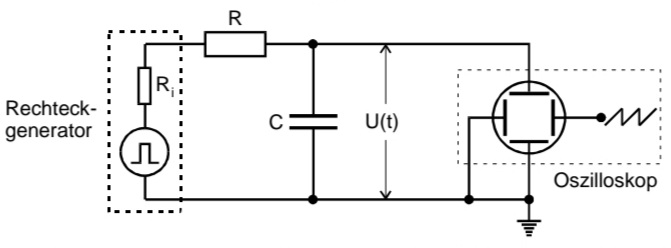
\includegraphics[width=0.75\textwidth]{plots/Schaltung1.png}
    \caption{Schaltung für den Austausch der Schwingungsenergie \cite{Versuchsanleitung}}
    \label{fig:schaltung1}
\end{figure}

\noindent Der Versuch wird mit einem Rechtecksignal mit $300$ bis $500 \:\si{\hertz}$ am Signalgenerator durchgeführt.
Zunächst wird der Schaltplan gemäß \autoref{fig:schaltung1} aufgebaut. Nun werden in Abhängigkeit der verstellbaren Kopplungskapazität $C_{\text{K}}$ die 
Schwingungsmaxima einer Schwebung gezählt. Es wird außerdem die Zeit einer Schwebungsperiode gemessen.
Der Vorgang wird für alle möglichen Kopplungskapazitäten auf dem Schaltkasten wiederholt.

\subsection{Fundamentalschwingung}
% Schaltplan umgestell gedöns, das ich beim besten willen nicht mehr weiß
Das Oszilloskop wird wieder auf die XY-Funktion umgestellt, damit wird mit Lissajous-Figuren die Frequenzen der Fundamentalschwingungen gemessen. 
Es wird ein Sinussignal mit der Resonanzfrequenz am Generator eingestellt. Im Anschluss werden die Frequenzen in Abhängigkeit der Kopplungskapazität 
gemessen, bei denen die Lissajous-Figuren auf eine Gerade abgebildet werden. Der Vorgang wird, analog zum Aufgabenteil zuvor, für alle möglichen 
Kopplungskapazitäten auf dem Schaltkasten wiederholt. 

\subsection{Strömungsverlauf}
Der Schaltplan bleibt wie bei der Messung der Fundamentalschwingungen. Am Spannungsgenerator wird mithilfe des Wobbelgenerators ein Frequenzzähler
eingeschaltet. Dieser geht die Freqenzen von 20.00 kHz bis 50.00 kHz innerhalb von 0.02 Sekunden durch und bildet die Spannungsmaxima somit in
Abhängigkeit der Frequenzen ab. Es werden die Position und der Wert der Spannungsmaxima aufgenommen. Die Messreihe wird wieder für alle
möglichen Kopplungskapazitäten auf dem Schaltkasten wiederholt.